\documentclass[UTF8,12pt]{article} % 12pt 为字号大小
\usepackage{amssymb,amsfonts,amsmath,amsthm,latexsym}
\usepackage{subfigure}
\usepackage{float}
\usepackage{graphicx}
%\usepackage{fontspec,xltxtra,xunicode}
%\usepackage{times}

%----------
% 定义中文环境
%----------

\usepackage{xeCJK}

\setCJKmainfont[BoldFont={SimHei},ItalicFont={KaiTi}]{SimSun}
\setCJKsansfont{SimHei}
\setCJKfamilyfont{zhsong}{SimSun}
\setCJKfamilyfont{zhhei}{SimHei}
\setCJKfamilyfont{zhkai}{KaiTi}
\setCJKfamilyfont{zhfs}{FangSong}
\setCJKfamilyfont{zhli}{LiSu}
\setCJKfamilyfont{zhyou}{YouYuan}

\newcommand*{\songti}{\CJKfamily{zhsong}} % 宋体
\newcommand*{\heiti}{\CJKfamily{zhhei}}   % 黑体
\newcommand*{\kaiti}{\CJKfamily{zhkai}}  % 楷体
\newcommand*{\fangsong}{\CJKfamily{zhfs}} % 仿宋
\newcommand*{\lishu}{\CJKfamily{zhli}}    % 隶书
\newcommand*{\yuanti}{\CJKfamily{zhyou}} % 圆体

%----------
% 版面设置
%----------
%首段缩进
\usepackage{indentfirst}
\setlength{\parindent}{2em}

%行距
\renewcommand{\baselinestretch}{1.4} % 1.4倍行距

%页边距
\usepackage[a4paper]{geometry}
\geometry{verbose,
  tmargin=2cm,% 上边距
  bmargin=2cm,% 下边距
  lmargin=3cm,% 左边距
  rmargin=3cm % 右边距
}


%----------
% 其他宏包
%----------
%图形相关
\usepackage[x11names]{xcolor} % must before tikz,x11names defines RoyalBlue3
\usepackage{graphicx}
\usepackage{pstricks,pst-plot,pst-eps}
\usepackage{subfig}
\def\pgfsysdriver{pgfsys-dvipdfmx.def} % put before tikz
\usepackage{tikz}

%原文照排
\usepackage{verbatim}

%网址
\usepackage{url}

%----------
% 习题与解答环境
%----------
%习题环境
\theoremstyle{definition} 
\newtheorem{exs}{习题}

%解答环境
\ifx\proof\undefined\
\newenvironment{proof}[1][\protect\proofname]{\par
\normalfont\topsep6\p@\@plus6\p@\relax
\trivlist
\itemindent\parindent
\item[\hskip\labelsep
\scshape
#1]\ignorespaces
}{%
\endtrivlist\@endpefalse
}
\fi

\renewcommand{\proofname}{\it{证明}}


%==========
% 正文部分
%==========

\begin{document}

\title{基于卷积神经网络的图像分类系统}
\author{SJTU}
%\date{} % 若不需要自动插入日期,则去掉前面的注释;{ } 中也可以自定义日期格式
\maketitle

\section{任务介绍}
CIFAR-10 数据集由60000张图片组成,每张图片的大小为32 $\times$ 32,RGB三通道。整个数据集都被标记为十个标签的一种。数据集在下载后已经被分为5个训练Batch和1个测试Batch。每个Batch都包含10000张图片。\cite{krizhevsky2009learning}

\subsection{工作概述}
此Project进行CIFAR-10数据集的图像分类,需要基于CNN。由于数据集已经进行打包,我们直接使用数据集的训练集-测试集分类方法。需要完成的工作包括数据预处理,设计模型,设计训练策略,实际训练,进行训练总结(以文字和可视化的形式)。模型使用Pytorch工具,基于\url{https://pytorch.org/tutorials/beginner/blitz/cifar10_tutorial.html}. \\
\indent
在没有使用额外数据以及预训练模型的前提下,我们设计的模型准确率达到了90\%,参数大小为83MB. 此外,按照要求,随机数种子被设为2021,便于审阅我们的结果。

\subsection {相关工作}
在\url{https://paperswithcode.com/sota/image-classification-on-cifar-10} 中含有使用此数据集模型排名。主流模型包括Transformer\cite{dosovitskiy2021image},ResNet\cite{kolesnikov2020big},EfficientNet\cite{tan2021efficientnetv2},DCN\cite{sousa2021cnn},ResNeXt\cite{Li_2019_CVPR}等。\\
\indent 从2012年有记录以来,年度最佳模型的准确率从88.8\%提高到了99.5\%。发表于2021CVPR的ViT-H/14将准确率提高到了99.5\%\cite{dosovitskiy2021image},而使用CNN的FlexConv在达到92.2\%以上准确率的同时\cite{romero2021flexconv},保证了自己的参数大小约为0.67MB,约为准确率最高的模型的$\frac{1}{1000}$.


\section{数据处理}
我们采取了以下数据预处理方式:
\begin{itemize}
\item 随机裁剪(Random Crop)
\item 随机水平翻转(Random Horizontal Flip)
\item 随机仿射变换(Random Affine)
\item 颜色抖动(Color Jitter)
\end{itemize}


\begin{figure}[H]
	\centering
	\subfigure[原始数据集]{
		\centering
		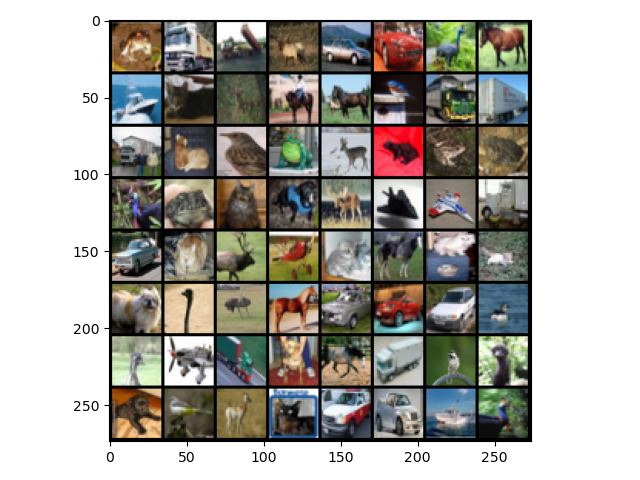
\includegraphics[width=0.4\linewidth]{original_dataset}
	}
	\subfigure[扩充数据集1]{
		\centering
		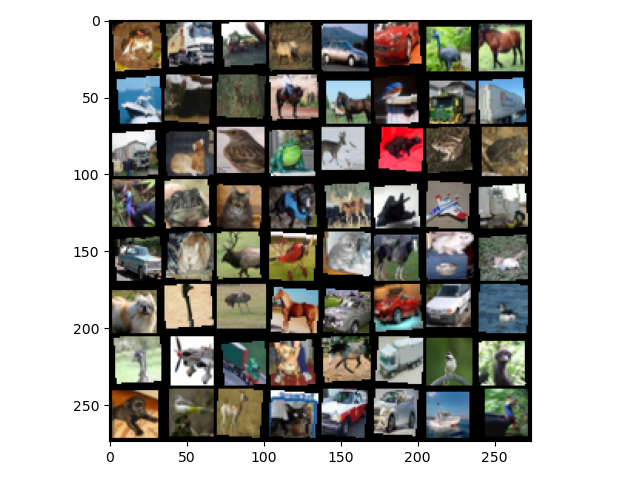
\includegraphics[width=0.4\linewidth]{augment1}
	}
	\subfigure[扩充数据集2]{
		\centering
		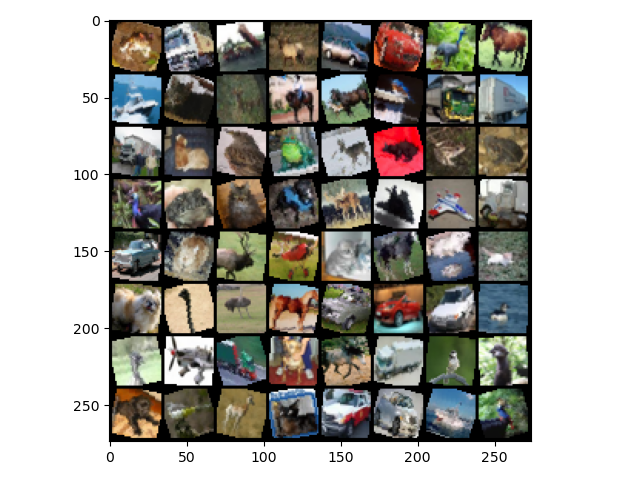
\includegraphics[width=0.4\linewidth]{augment2}
	}
	\subfigure[扩充数据集3]{
		\centering
		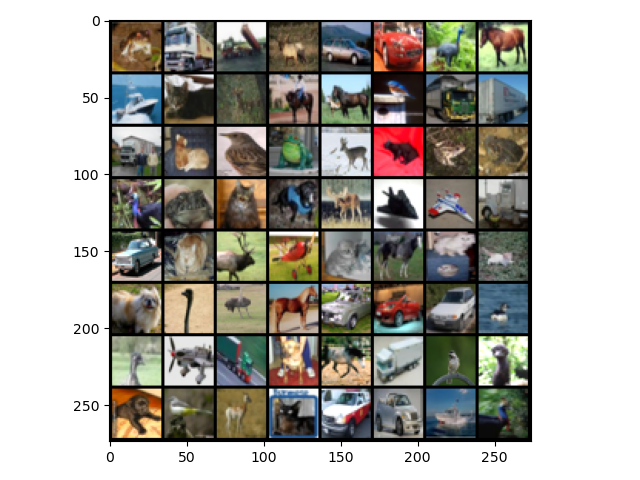
\includegraphics[width=0.4\linewidth]{augment3}
	}
	\caption{原始数据集,扩充数据集1(随机裁剪+随机水平翻转+随机仿射变换),扩充数据集2(随机放射变换),扩充数据集3(颜色抖动)}
\end{figure}
通过图像增强,我们扩充了数据集,为训练提供了更多样本。
\section{模型设计}
\subsection{架构选择}
ResNet是时下应用最广泛的基于CNN的图像分类模型。\cite{he2015deep} 他的提出让CNN的层数由原来的不到十层提高到了上百层甚至上千层。人们发现随着CNN层数的增多,模型准确度反而下降。而这不能用过拟合来解释(因为训练集和测试集的Loss都同步上升),而随着BN大部分解决了梯度消失/爆炸问题后,模型退化问题仍然存在。
\\ 
\indent
ResNet提出了Shortcut方法,引入了恒等映射,让模型拥有了“什么都不做”的选择,有效防止了更多的层数带来的信息丢失。而更多的层数为分层学习提供了可能,每一层学到更细化的特征,提高了模型的表达能力。
\\ 
\indent
因此,我们的模型是基于ResNet的基本框架进行调参的。在ResNet论文\cite{he2015deep}中提出了5种ResNet模型,即ResNet18,ResNet34,ResNet50,ResNet101,ResNet152. 数字代表的是层数,我们尝试复现了以下框架。\ref{Fig.resnet1}
%% 一张
\begin{figure}[h] %H为当前位置,!htb为忽略美学标准,htbp为浮动图形
	\centering %图片居中
	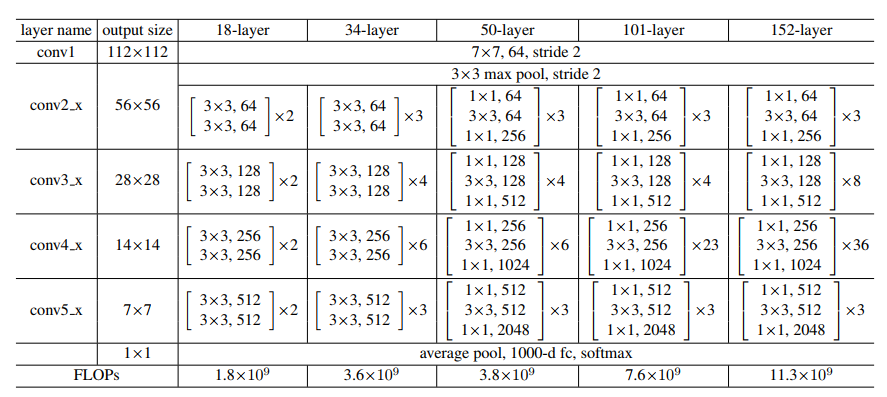
\includegraphics[width=0.7\textwidth]{resnet.png} %插入图片,[]中设置图片大小,{}中是图片文件名
	\caption{ResNet 论文中给出的模型结构} %最终文档中希望显示的图片标题
	\label{Fig.resnet1} %用于文内引用的标签
\end{figure}
\\
\indent
但是,在层数升至50层以上时,即使使用多块RTX3080显卡进行训练,也需要数小时甚至十余小时才能完成训练。我们优先将有限的资源使用在了低层数的ResNet上。特别对ResNet18(便于调参与快速训练查看结果)以及ResNet50(较好的平衡了层数和训练资源)进行了调参和训练。

\subsection{优化器}
常见的优化器包括SGD,Adam,LAMB. 大部分的卷积神经网络都采用了SGD作为优化器,少许采用了Adam作为优化器。上述的Benchmark Top1\cite{dosovitskiy2021image}模型指出了在ResNet50模型中,Adam和SGD的表现是几乎没有任何差别的。因此,我们简单地采用阅读论文时的观察和建议,选择了SGD作为优化器。


\section{训练计划}
\subsection{平台}
使用了矩池云平台进行训练,租用了至多4块RTX3080 Ti显卡,CPU为8 $\times$ Xeon E5-2682 v4核心,86G内存。系统环境为Python3.7,CUDA 11.1,cuDNN 8.0.5,Pytorch 1.8.1, Horovod 0.22.1,Ubuntu 18.04.

\subsection{Baseline}


\section{模板介绍}
这个模板是UTF-8编码的,使用xeCJK宏包,中英文混排更美观,但编译速度稍慢。注意:该模板只能用xelatex编译。常用逻辑符号命令:
\begin{center}
\begin{tabular}{|c|c|c|}
\hline
名称      & 符号                   & 命令 \\
\hline
否定      & $\neg$                & \verb|\neg| \\
合取      & $\land$               & \verb|\land| \\
析取      & $\lor$                & \verb|\land| \\
蕴含      & $\to$                 & \verb|\to| \\
推出      & $\Rightarrow$         & \verb|\Rightarrow| \\
实质蕴涵   & $\supset$             & \verb|\supset| \\
双蕴含     & $\leftrightarrow$     & \verb|\leftrightarrow| \\
等价      & $\equiv$              & \verb|\equiv| \\
存在量词   & $\exists$             & \verb|\exists| \\
全称量词   & $\forall$             & \verb|\forall| \\
必然      & $\Box$                & \verb|\Box| \\
可能      & $\Diamond$            & \verb|\Diamond| \\
可满足,真  & $\models$            & \verb|\models| \\
语义后承   & $\vDash$,$\nvDash$   & \verb|\vDash,\nvDash| \\
句法后承   & $\vdash$,$\nvdash$   & \verb|\vdash,\nvdash| \\
属于      & $\in$,$\notin$       & \verb|\in,\notin| \\
真包含于   & $\subset$             & \verb|\subset| \\
包含于     & $\subset$            & \verb|\subset| \\
不等于     & $\neq$               & \verb|\neq| \\
小于等于   & $\leq$               & \verb|\leq| \\
大于等于   & $\geq$               & \verb|\geq| \\
下省略    & $\ldots$              & \verb|\ldots| \\
中省略    & $\cdots$              & \verb|\cdots| \\
对角省略  & $\ddots$              & \verb|\ddodts| \\
\hline 
\end{tabular}
\end{center}
更多符号对应的命令请参见:
\begin{itemize}
  \item \url{https://oeis.org/wiki/List_of_LaTeX_mathematical_symbols}或
  \item \url{https://www.ctan.org/tex-archive/info/symbols/comprehensive/}
\end{itemize}


\section{中文字体}

\subsection{字体切换}
默认字体为宋体。我们可以这样来改变中文字体:\heiti 从现在起是黑体。\kaiti 从现在起是楷体。\fangsong 从现在起是仿宋。\lishu 从现在起是隶书。\yuanti 从现在起是圆体。\songti 从现在起又是宋体。

\subsection{字体强调}
加粗字体自动变为黑体:\bf{粗体},加斜或强调字体自动变成楷体:\it{斜体},\emph{强调}。


\section{习题环境}

\begin{exs}
请证明勾股定理。
\end{exs}
\begin{proof}
这是证明。末尾后会自动添加方块以示结束。
\end{proof}

\begin{exs}
请计算 $1+2+\ldots +100$。
\end{exs}
\begin{proof}[解答]
这是解答。末尾后会自动添加方块以示结束。
\end{proof}

\nocite{*}
\bibliographystyle{acm}
\bibliography{ref.bib}
\end{document}
